\chapter{Введение в проблему. Исторический обзор.\todo{Переработать и убрать во Введение?...}}\label{ch:ch1}

Критически важным (\textbf{mission-critical}) фактором системы является любой фактор
(компонент, оборудование, персонал, процесс, процедура, программное обеспечение и т. д.),
необходимый для ведения бизнеса или для его организации.
Отказ или срыв одного из факторов приведет к серьезному воздействию на бизнес-операции или на организацию
и даже может вызвать социальные потрясения и катастрофы.

Приведены примеры катастроф, приведших к человеческим жертвам, большим экономическим потерям,
по причине наличия ошибок или недочетов в программно-аппаратных комплексах.


\section{Ошибки программного обеспечения с летальными исходами и финансовыми потерями}

\textbf{Серия крушений новейших самолетов Boeing~737~MAX.}
Крушение самолётов Boeing~737~MAX из-за ошибки в некорректной работе системы MCAS\footnote{Maneuvering Characteristics Augmentation System ---
    система улучшения летных характеристик.},
призваной \underline{незаметно} помогать пилоту управлять самолётом в ручном режиме (при отключении автопилота),
вместо этого при неисправности одного из датчиков угла атаки MCAS принудительно отправила аваиалайнер в пике
(две катастрофы, общее количество жертв 346:
    29 октября 2018 года возле Джакарты --- 189 человек;
    10 марта 2019 года в Эфиопии --- 149 пассажиров и 8 членов экипажа).
Убытки корпорации в первой половине 2020 года порядка 15 млрд долларов;
компенсация семьям погибших в 2019 году --- 5.6 млрд долларов;
в конце января 2020 года переговоры с банками о взятии займа на сумму в 10 млрд долларов для покрытия убытков от приостановки полетов Boeing~737~MAX;
порядка 5 млрд долларов на переподготовку пилотов на тренажерах перед возобновлением эксплуатации авиалайнеров;
отставка генерального директора корпорации Денниса Мюленбурга.
% https://www.boeing.com/commercial/737max/737-max-software-updates.page


\textbf{Передозировка с помощью аппарата Therac-25.}
Аппарат лучевой терапии Therac-25 стал причиной как минимум шести передозировок радиации (июнь 1985 --- январь 1987 гг.),
некоторые пациенты получили дозы в десятки тысяч рад. Как минимум двое умерли непосредственно от передозировок \cite{journal:computer:1993:therac25}.
Внешний вид прибора показан на рисунке \ref{fig:therac25}.

\begin{center}
    \begin{figure}[hb!]
        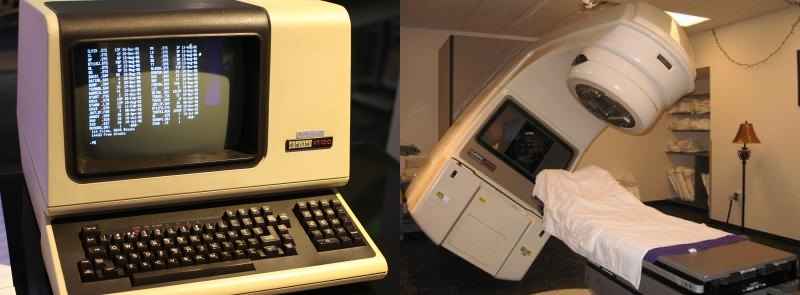
\includegraphics[width=.7\textwidth]{therac25-console}
        \caption{Therac 25}\label{fig:therac25}
        %
        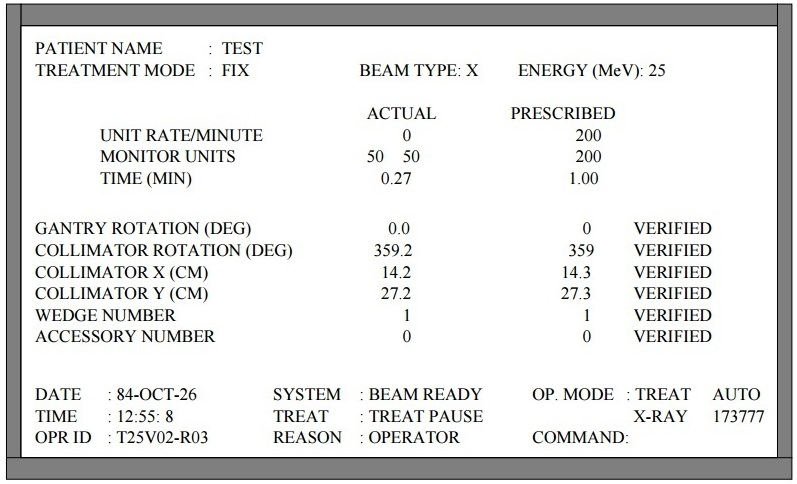
\includegraphics[width=.7\textwidth]{therac25-screenshot}
        \caption{Консоль Therac 25}\label{fig:therac25_console}
    \end{figure}
\end{center}
    
    
\textbf{Блэкоут.}
В 2003 году\footnote{\url{https://m.habr.com/ru/company/mailru/blog/370153/}}.


\textbf{Третья мировая война.} % https://m.habr.com/ru/company/mailru/blog/485612
Запуск балистических ракет в 1983 году (там же).


\textbf{Перелет через линию смены дат.}
Смена часового пояса у истребителей F-22. 


\textbf{Катастрофа при первом полете Ariane~5.}
Первый испытательный полет в 1996 году Ariane~5 \cite{journal:open_system:1998_adjaev}\footnote{\url{http://www.osp.ru/os/1998/06/179592}},
европейской одноразовой тяжёлой ракеты-носителя семейства Ариан,
предназначеной для выведения полезной нагрузки на низкую опорную орбиту или геопереходную орбиту. 
%
Ракета-носитель была подорвана на 34-й секунде полёта по причине неисправности в управляющем программном обеспечении.
Конвертация данных из 64-разрядного числа с плавающей запятой в 16-разрядное привела к зависанию компьютера.
Процедура на языке Ada, обрабатывающая эту исключительную ситуацию, была исключена из соображений сохранения производительности системы.
%
Это считается самой дорогостоящей компьютерной ошибкой в истории.
Отметим, что всю цепь событий удалось полностью воспроизвести с помощью компьютерного \textbf{моделирования},
что вкупе с материалами других исследований и экспериментов позволило полностью выявить причины и обстоятельства катастрофы.